\documentclass{article}
\usepackage[utf8]{inputenc}
\usepackage{graphicx}
	\DeclareGraphicsExtensions{.png, .jpeg}
\usepackage[top=1in, bottom=1in, left=1in, right=1in]{geometry}

\title{Autonomoboro \\ Lab05: Line Following}
\author{Bandith Phommounivong, Terence Henriod}
\date{\today}

\begin{document}

\maketitle

\begin{abstract}
A dicussion of a robot designed to follow a line and then return home when called for.
\end{abstract}

\newpage

\section{Robot Design}

The challenge this time involved 

\subsection{Hardware Configuration}
This

	\begin{figure}[h!]
	\centering
	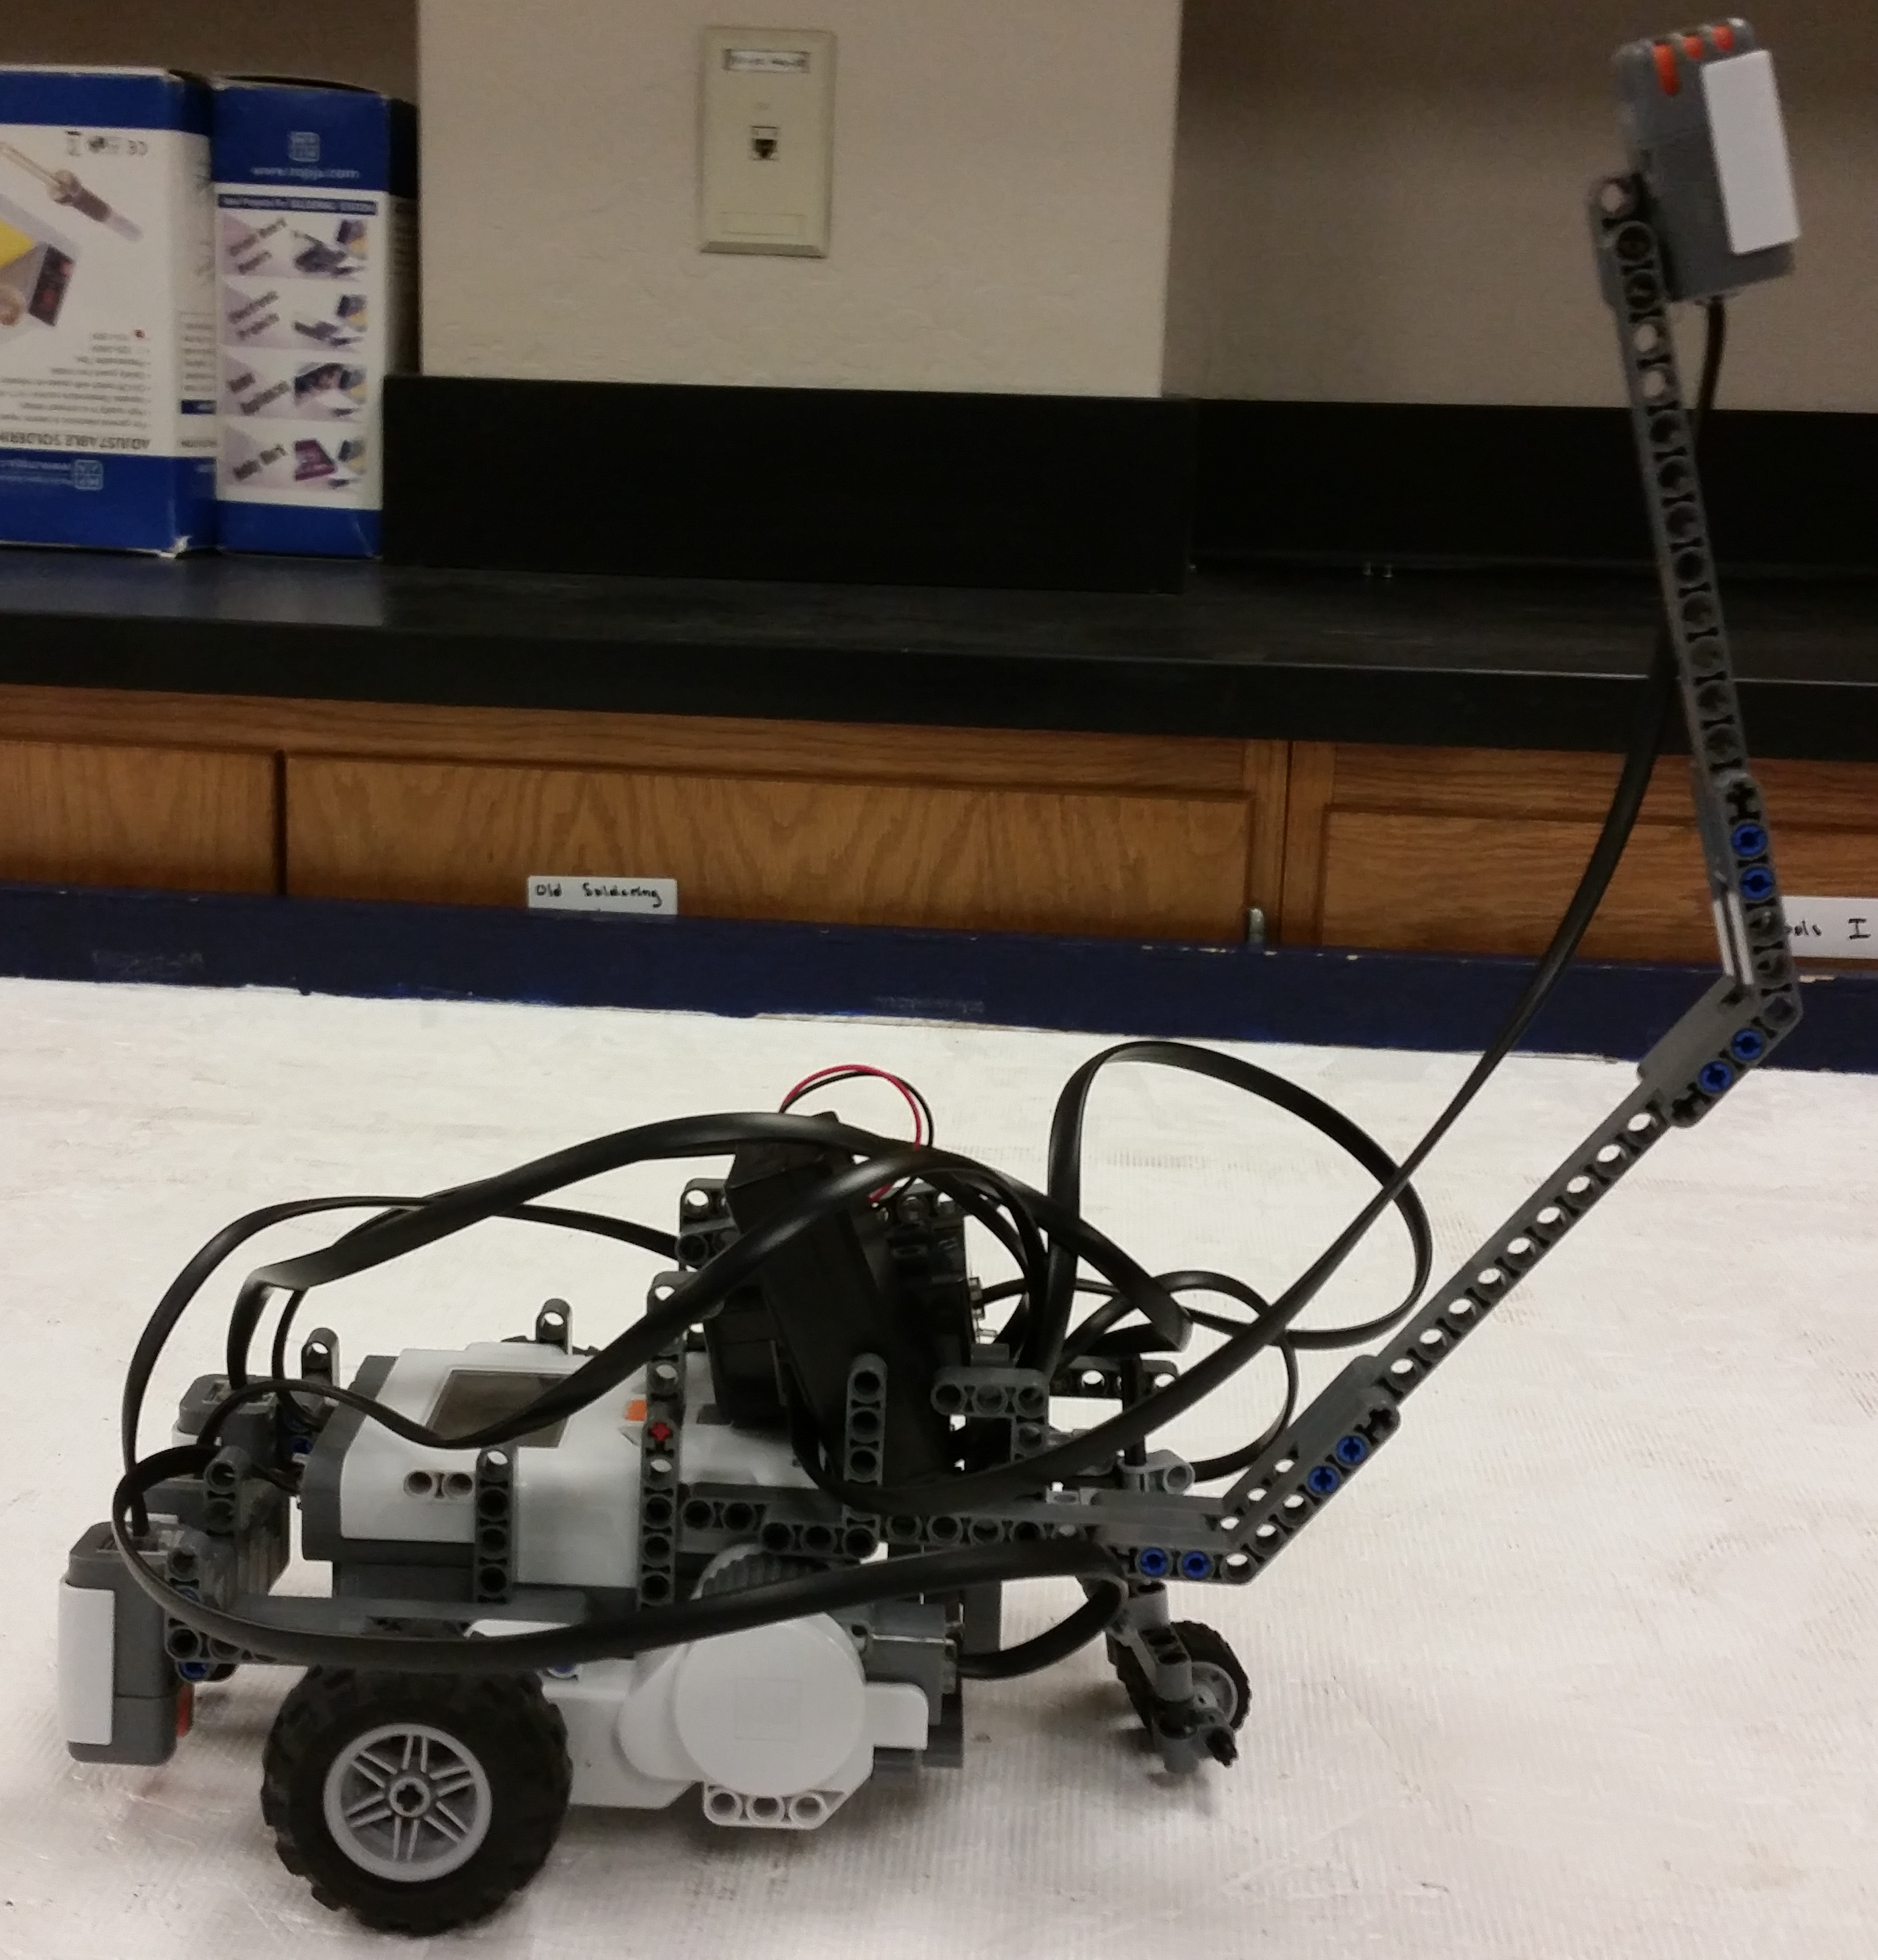
\includegraphics[width = 0.4\textwidth]{bad_robot}
        % extension usually unnecessary when specifying file
	\caption{A bad robot.}
	\label{fig:bad_robot}
	\end{figure}

    \begin{figure}[h!]
    \centering
    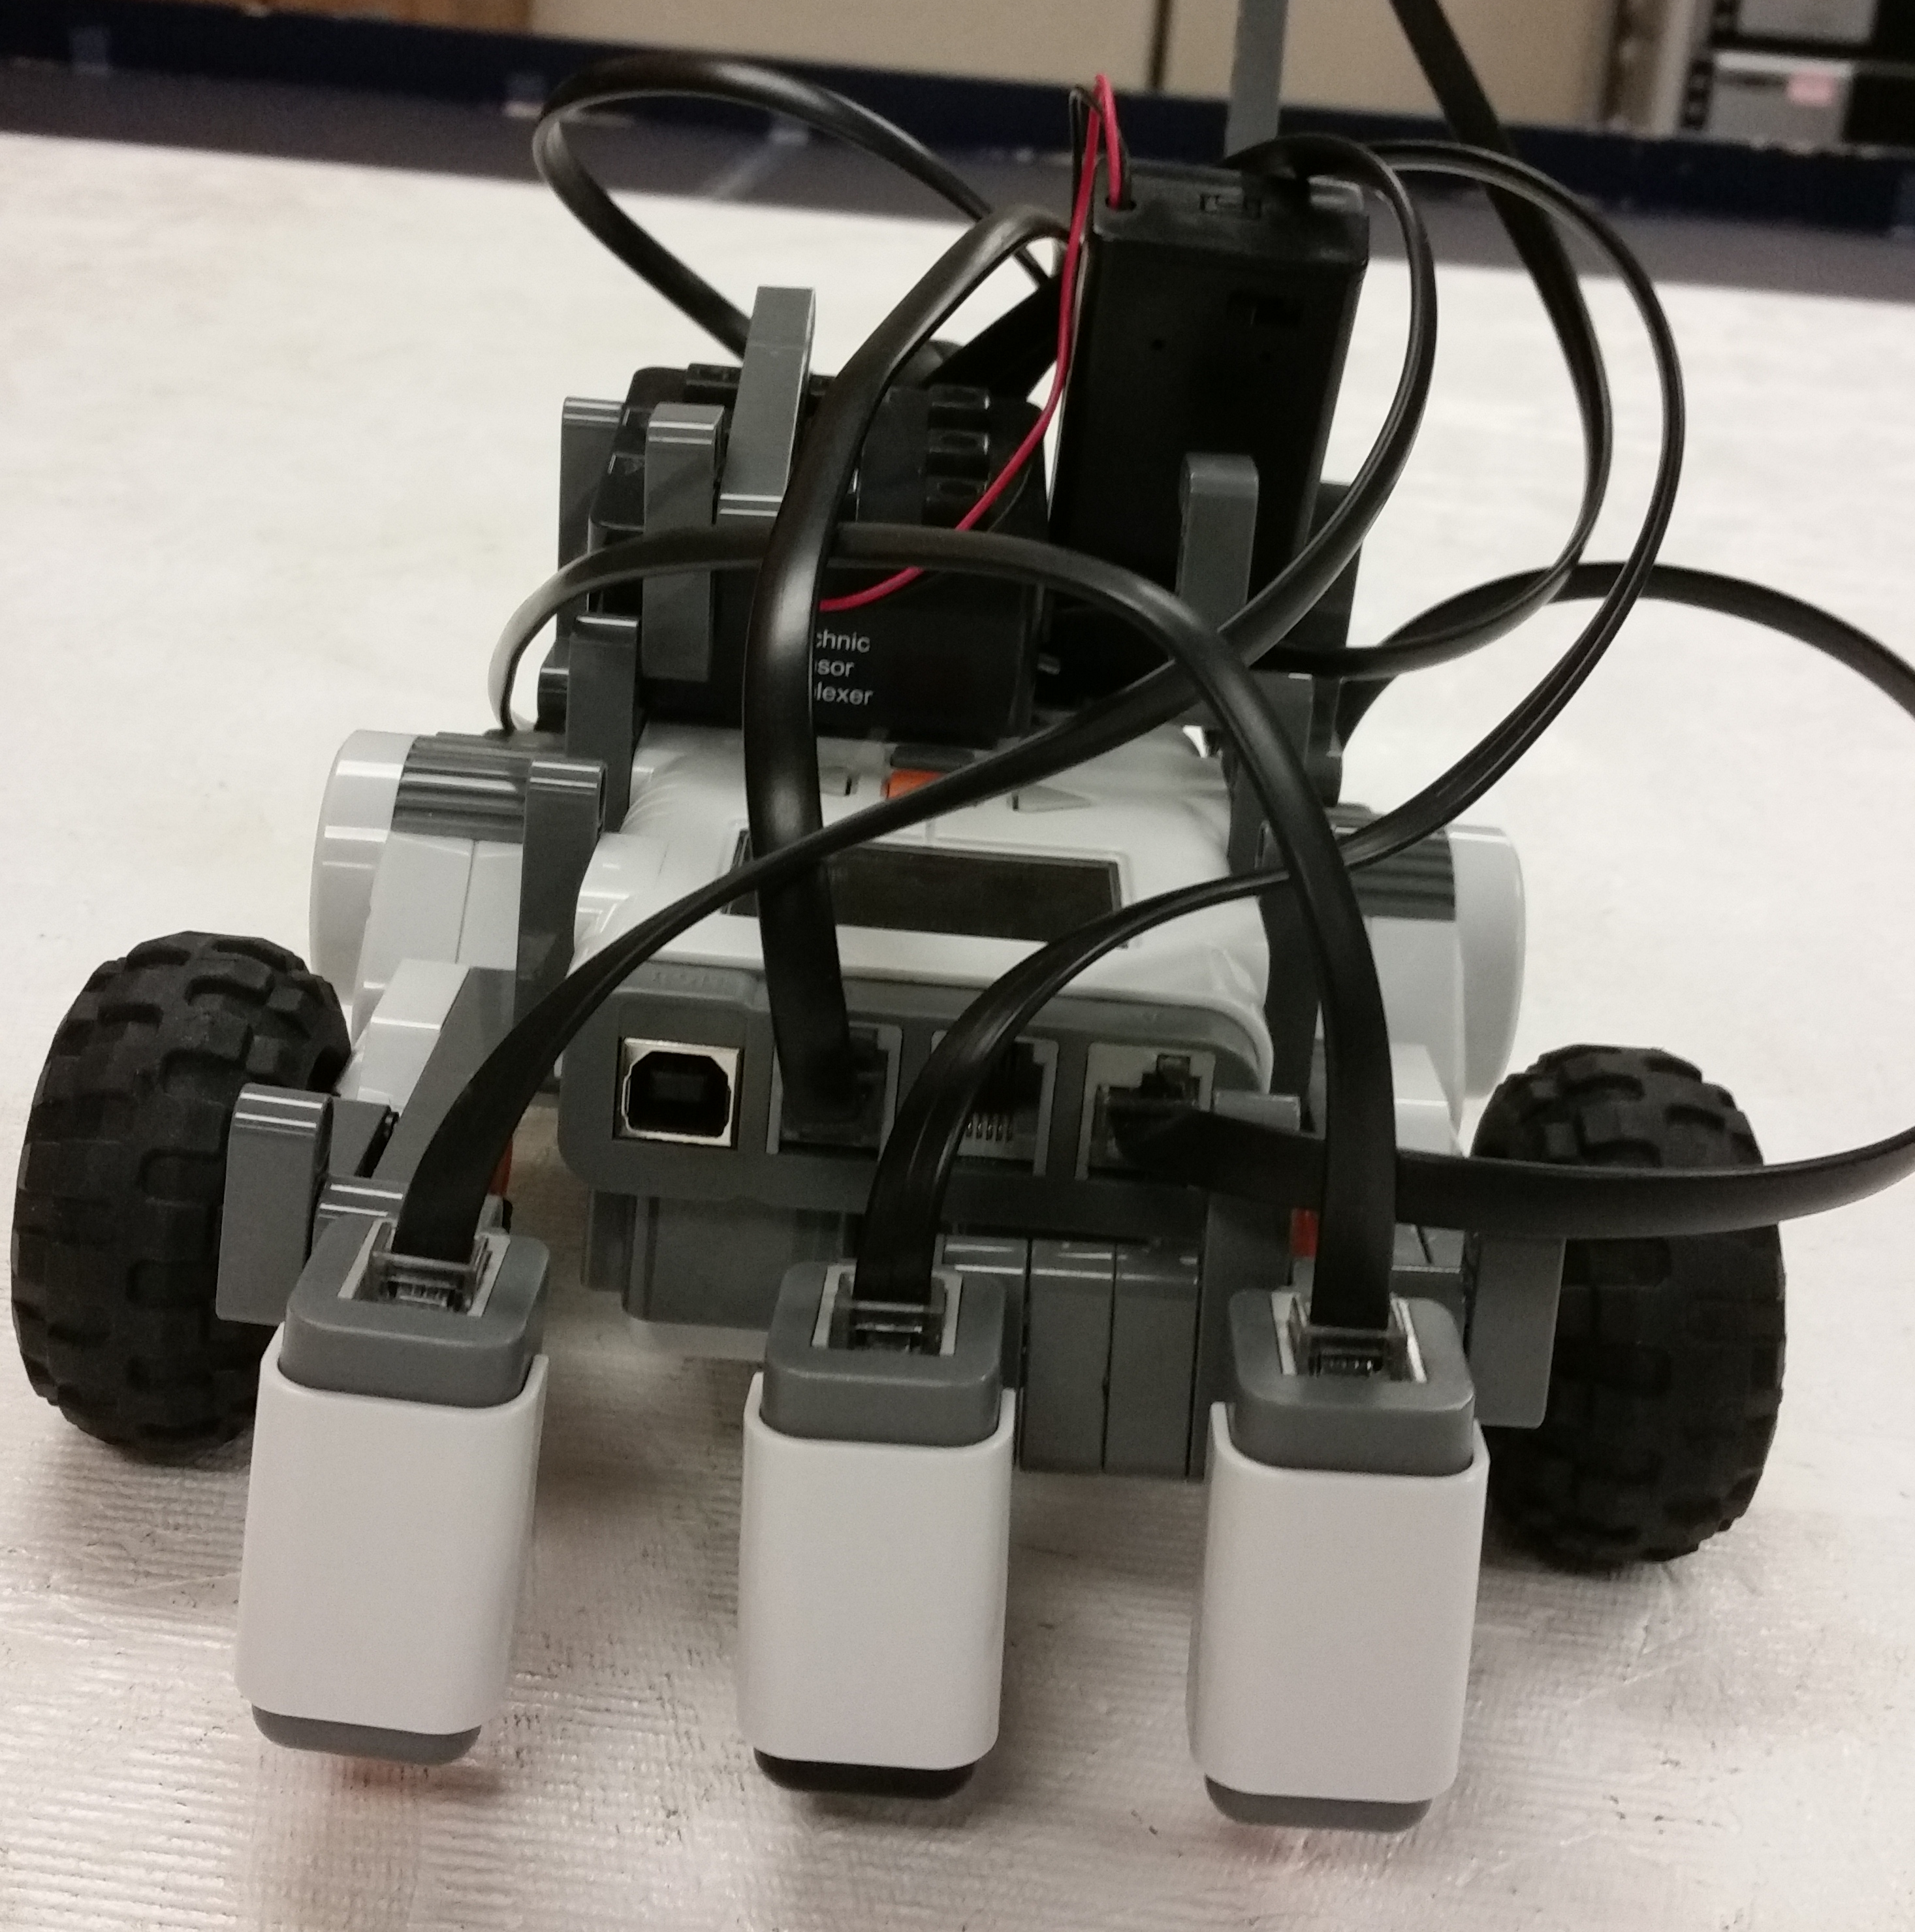
\includegraphics[width = 0.4\textwidth]{bad_robot_front_view}
        % extension usually unnecessary when specifying file
    \caption{A bad robot as seen from the front.}
    \label{fig:bad_robot_front_view}
    \end{figure}


    \begin{figure}[h!]
    \centering
    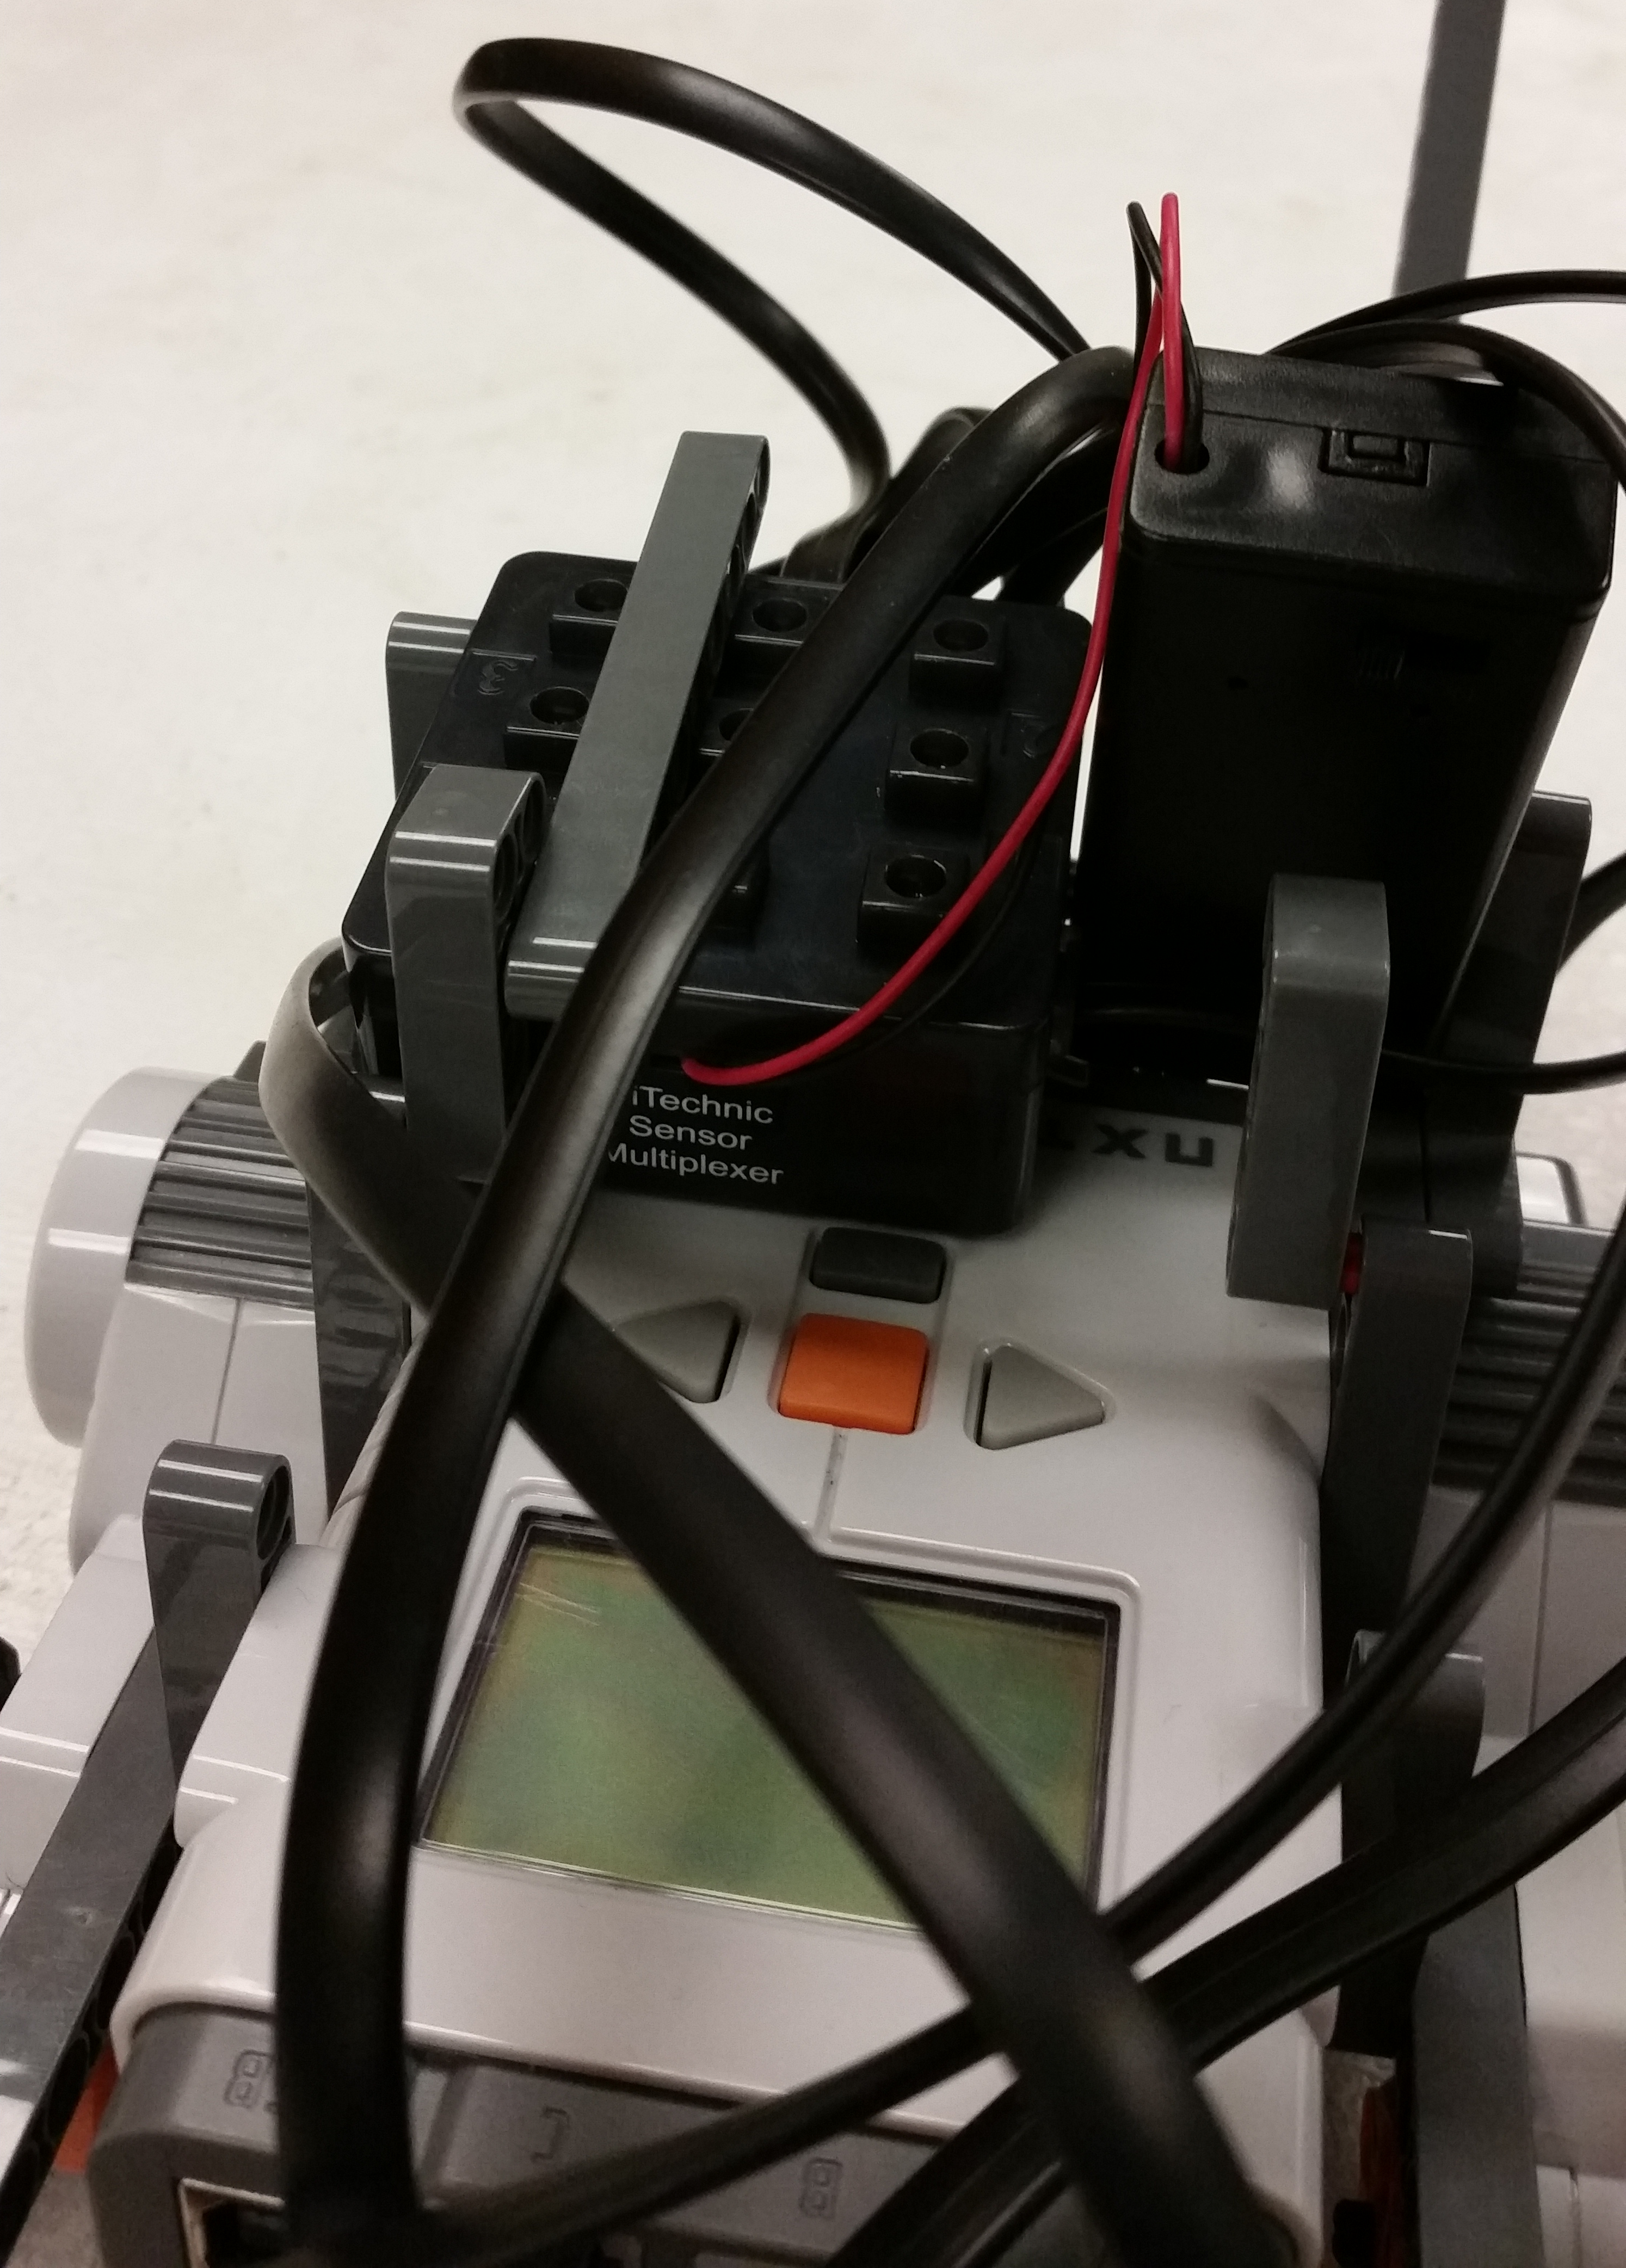
\includegraphics[width = 0.4\textwidth]{bad_robot_mux}
        % extension usually unnecessary when specifying file
    \caption{A bad robot.}
    \label{fig:bad_robot_mux}
    \end{figure}

\subsection{Software Design}


\section{Implementation Problems and Their Solutions}


\section{Unsolved Problems}


\end{document}
